\documentclass{article}
\usepackage{amsmath}
\usepackage{graphicx}
\usepackage{enumerate}
\usepackage{natbib}
\usepackage{url} % not crucial - just used below for the URL 

%\pdfminorversion=4
% NOTE: To produce blinded version, replace "0" with "1" below.
\newcommand{\blind}{0}

% DON'T change margins - should be 1 inch all around.
\addtolength{\oddsidemargin}{-.5in}%
\addtolength{\evensidemargin}{-1in}%
\addtolength{\textwidth}{1in}%
\addtolength{\textheight}{1.7in}%
\addtolength{\topmargin}{-1in}%

%My
\usepackage{amssymb}
\usepackage{amsfonts}
\usepackage{enumerate}
\usepackage{algorithm}
\usepackage{multirow}
%\usepackage{algorithmic}
\usepackage{lmodern}
\usepackage{setspace}
\usepackage{hyperref}
\usepackage{xcolor}
\usepackage{amsthm}
\usepackage{hyperref}
\usepackage{booktabs}
\usepackage{enumitem}

\newtheorem{theorem}{Theorem}[section]
\newtheorem{proposition}[theorem]{Proposition}
\newtheorem{lemma}[theorem]{Lemma}
\newtheorem{corollary}[theorem]{Corollary}
\newtheorem{definition}[theorem]{Definition}
\newtheorem{assumption}[theorem]{Assumption}
\newtheorem{remark}[theorem]{Remark}

\usepackage{kotex}
\usepackage{xcolor}
%\usepackage{algorithm}
\usepackage{algpseudocode}

\def\spacingset#1{\renewcommand{\baselinestretch}%
{#1}\small\normalsize} \spacingset{1}


\title{Fair representation learning with sup IPM}
\author{Yongdai Kim}
\date{July 2026}

\begin{document}

\maketitle


\section{Story}

\begin{itemize}
    \item Fair representation learning에서 sensitive variable이 contin한 경우
    \item 이 경우 GDP를 보장하는 방법론들이 제안되었다.
    \item 그러나 discrete 경우에서 볼 수 있다 싶이 DP는 원래 for all s에 대해서 보장되어야 한다.
    \item 이것을 conti로 자연스럽게 확장하면 expection이 아닌 sup을 고려하게 된다.
    \item 우리는 그래서 $L_{\infty}$ GDP를 제안한다.
    \item 기존에 GDP를 보장하는 fair representation에 FREM이 있었다.
    \item 이를 확장한
\end{itemize}

\section{Introduction}



\begin{itemize}
 \item The problem is how to  learn fair representation when the sensitive variable is continuous.
 \item Previously, regularized method and binning이 사용되었지만 문제가 있었다.
 \item \cite{kong2025fair} attacked this problem by introducing the EIPM.
 \item They used MMD for the IPM.
 \item There are at least three problems in the fair-EIPM.
   \begin{itemize}
     \item The class of discriminator for MMD would be limited to infinitely differentialble functions
     (e.g. Gaussian kernel)  or having a special low dimensional structure (e.g. tensor product kernel).
     This limitation results in a guarantee of fairness only for limited functions (e.g. functions beloing
     to a given class of discriminators). 
     \item Sensitive attribute가 continuous한 경우 Demographic parity는 모든 $s$에 대해서 보장 되어야 하므로 이것을 continous로 확장할 시에 sup을 생각하는것이 자연스럽다.
     \item $L_{\infty}$ generalized demographic parity ($L_{\infty}$ GDP) 제안한다
     \item 이것을 보장하는 measure로써 sup IPM을 고려함.
     \item The fairness is guaranteed in the terms of $\ell_1$ norm with respect to the sensitive variable.
      The sup-norm fairness guarantee would be needed in practice.
      \item Computation is demandning (i.e. $O(n^3)$) and not easy to be modified for minibatch learning.
   \end{itemize}
 \item In this paper, we propose an adversarial learning framework which has the following advantages:
   \begin{itemize}
   \item 새로운 $L_{\infty}$ GDP 제안
       \item It guarantees the fairness for any Holder smooth functions which are bigger than the RKHS (the
       set of discriminators for MMD).
       \item The fairness is guaranteed by the sup-norm with resepect to the sensitive variable. 
       \item Minibatch-learning is possible and so it can be scaled up easily.
   \end{itemize}
\end{itemize}

\section{Review of Fair representation learning algorithms with continuous sensitive attributes}

\begin{itemize}

    \item FREM
    \item Relu-IPM
\end{itemize}


\section{Sup-IPM for fair representation learning}

\begin{itemize}
    \item $g_\gamma: \mathcal{X} \rightarrow \mathcal{Z}:$ a feature mapping parameterized by $\gamma\in \Gamma.$
    \item $\mathbb{P}_{g_\gamma(X)|S=s}$ be the population conditional distribution of $g_\gamma(X)$ given $S=s.$
    \item Suppose that we know $\mathbb{P}.$ Then, we can find $\gamma$ by minimzing
    $$\sup_{s\in \mathcal{S}}\text{IPM}_{\mathcal{V}}(\mathbb{P}_{g_\gamma(X)|S=s}, \mathbb{P}_X),$$
    where $\mathcal{V}$ is the set of discriminators.
    \item Consider a $C$-class classification problem. Suppose that
    $\mathbb{P}(Y=c|x)=f_c(g_\gamma(x))$ for some $\gamma$ and $f_c, c\in [C].$
    If $\text{supIPM}_{\mathcal{V}} (g_\gamma)=\delta$ and $f_c\in \mathcal{V}$ for all $c\in [C],$ then
    we have
    \begin{equation}
    \label{eq:supfair}
    \sup_s \sup_{c} |\mathbb{P}(Y=c|X=x,S=s) - \mathbb{P}(Y=c|X=x)| \le \delta.
    \end{equation}
    That is, by controlling the supIPM, we can control the fairness of any classifier constructed
    on the top of any fair representation.
    \item Note that Fair-EIPM only guarantees 
    \begin{equation}
    \label{eq:expfair}
    \sup_c \mathbb{E}_S |\mathbb{P}(Y=c|X=x,S) - \mathbb{P}(Y=c|X=x)| \le \delta,
    \end{equation}
    which is weaker than (\ref{eq:supfair}) which guarantees that the classifier is fair for all $s,$
    while (\ref{eq:expfair}) only guarantees the fairness on average but does not guarantee the fairness
    on a given $S=s.$
    \item The size of the discriminator class is important for the fairness of the final classifier.
        The larger the the size is, the easier the final classifier is fair. MMD includes
        only super-smooth functions (e.g. Gaussian kernel) and/or functions having a special low dimensional structure (e.g. tensor product kernel). 
     \item We use the ReLU IPM which is known to cover Holder discriminators. That is, supIPM with ReLU discrimnators
     guarantees the fairness of Holder smooth classifiers which is much larger than the discriminator class
     induced by MMD with popularly used kernels. 
 \end{itemize}

\section{Estimation of supIPM}

\begin{itemize}
  \item To estimate the sup-IPM, we need to estimate $\mathbb{P}_{g_\gamma(X)|S=s}.$
  \item For this, we use a standard kernel density estimator: That is,
  $$\hat{\mathbb{P}}_{g_\gamma(X)|S=s} (\cdot)= \frac{\sum_{i=1}^n K_{h_n}(s-S_i) \delta_{g_\gamma(X_i)}(\cdot)}
    {D_n(s)},$$
  where $D_n(s)=\sum_{i=1}^n K_{h_n}(s-S_i).$  
  \item The corresponding estimator of IPM is
  $$\hat{\text{IPM}}_{\mathcal{V}}(g_\gamma,s)
    = \sup_{v\in \mathcal{V}} \left| \frac{\sum_{i=1}^n v(g_\gamma(X_i)) K_{h_n}(s-S_i)}{D_n(s)}
       -\frac{\sum_{i=1}^n v(g_\gamma(X_i))}{n}\right|,
  $$
  and so the corresponding supIPM becomes $\sup_s \hat{\text{IPM}}_{\mathcal{V}}(g_\gamma,s).$
\end{itemize}

\section{Computation}

\begin{itemize}
    \item Choice of the set of discriminators: ReLU
    \item Theoretical relation between the Holder discriminator and ReLU discriminator.
    \item Parallel computation with multiple initial choices
\end{itemize}

\section{Theoretical studies}

\begin{itemize}
    \item Let $\mathcal{H}_\alpha$ be the set of $\alpha$-Holder smooth functions.
    \item Let $\hat{\gamma}$ be a minimizer of the empirical supervised loss over the encoders and prediction heads satisfying the $\widehat{\text{supIPM}}_{\text ReLU}$ constraint.
    \item Then, we have
    $$\widehat{\text{supIPM}}_{\mathcal{H}}(g_{\hat{\gamma}})
    - \text{supIPM}_{\mathcal{H}}(g_{\hat{\gamma}}) = O_p(a_n)$$
    for $a_n\rightarrow 0.$
    \item A simple corollary is that for any $f\in \mathcal{H},$ we have
    $$\sup_s | \mathbb{E}(f(g_{\hat{\gamma}}(X)|S=s)-\mathbb{E}(f(g_{\hat{\gamma}}(X)))|
   = O_p(a_n).$$
   \item 이 때 $S$를 full domian ($[0,1]$)으로 사용하면 $a_n = (\frac{\log n}{n})^{\frac{1}{3}}$, $[t, 1-t]$ 이렇게 사용하면 $a_n = (\frac{\log n}{n})^{\frac{2}{5}}$가 되어서 mini-max optimal이 되지만 main 주장인 모든 $s \in S$에 대해서 불공정을 protect할 수 있다. 라고 주장하기가 애매해 질 것 같습니다.
\end{itemize}

\begin{figure}[t]
  \centering
  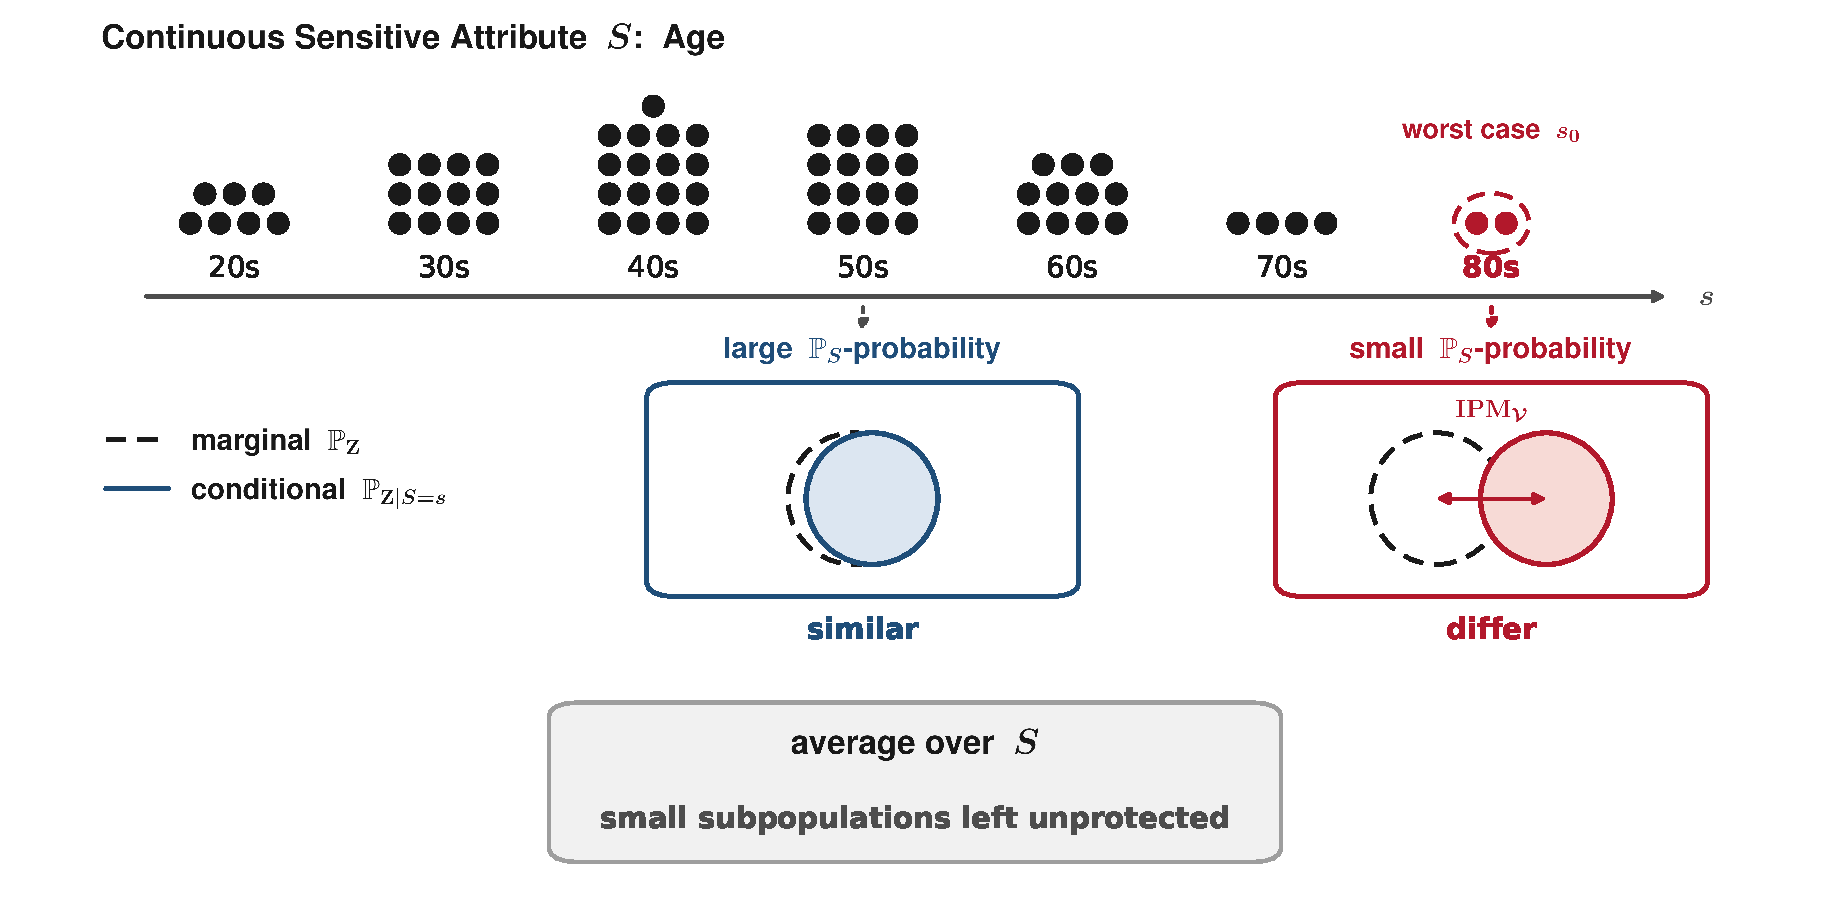
\includegraphics[width=\textwidth]{figures/motivation.pdf}
  \caption{The conditional and the marginal distribution of the representation coincide at a typical sensitive value and differ at $s_0$, a sensitive value where few observations lie.}
  \label{fig:motivation}
\end{figure}


 \bibliographystyle{plainnat}
\bibliography{bibliography}

\end{document}
